\documentclass[12pt,mathserif]{beamer}
 
% Define  CWRU specific color schemes
\definecolor{cwrublue}{RGB}{10,48,78}
\definecolor{cwrugrey}{RGB}{106,106,106}
%---------------------------------------

\mode<presentation>
{
  \usetheme{Boadilla}
  % \usecolortheme{dolphin}
  % Font themes
  \usefonttheme{serif}

  \setbeamercolor{palette primary}{bg=cwrublue,fg=white}
  \setbeamercolor{palette secondary}{bg=cwrublue,fg=white}
  \setbeamercolor{palette tertiary}{bg=cwrublue,fg=white}
  \setbeamercolor{palette quaternary}{bg=cwrublue,fg=white}
  \setbeamercolor{structure}{fg=cwrublue} % itemize, enumerate, etc
  \setbeamercolor{section in toc}{fg=cwrublue} % TOC sections

  % Override palette coloring with secondary
  \setbeamercolor{subsection in head/foot}{bg=cwrugrey,fg=white}
  % or ...

  %\setbeamercovered{transparent}
  % or whatever (possibly just delete it)
}

\usepackage[english]{babel}
% or whatever
\usepackage{mathptmx}
%\usepackage[latin1]{inputenc}
% or whatever

\usepackage{times}
\usepackage[T1]{fontenc}
% Or whatever. Note that the encoding and the font should match. If T1
% does not look nice, try deleting the line with the fontenc.

\title[Magnitude of odd-dimensional Euclidean balls]{On the asymptotic behavior of the magnitude function for odd-dimensional Euclidean balls}
\subtitle{Master's Thesis}

\author % (optional, use only with lots of authors)
{Stephen Shang Yi Liu}
% - Give the names in the same order as the appear in the paper.
% - Use the \inst{?} command only if the authors have different
%   affiliation.

\institute[CWRU] % (optional, but mostly needed)
{Department of Mathematics, Applied Mathematics and Statistics\and
Case Western Reserve University}
% - Use the \inst command only if there are several affiliations.
% - Keep it simple, no one is interested in your street address.

\date{March 19, 2020} % (optional, should be abbreviation of conference name)

% - Either use conference name or its abbreviation.
% - Not really informative to the audience, more for people (including
%   yourself) who are reading the slides online

\subject{Mathematics, Applied Mathematics and Statistics}
% This is only inserted into the PDF information catalog. Can be left
% out. 

% If you have a file called "university-logo-filename.xxx", where xxx
% is a graphic format that can be processed by latex or pdflatex,
% resp., then you can add a logo as follows:

%\pgfdeclareimage[height=0.5cm]{university-logo}{cwru-logo}
%\logo{\pgfuseimage{university-logo}}

% Delete this, if you do not want the table of contents to pop up at
% the beginning of each subsection:
%\AtBeginSubsection[]
%{
%  \begin{frame}<beamer>{Outline}
%    \tableofcontents[currentsection,currentsubsection]
%  \end{frame}
%}

% If you do not wish to uncover everything in a step-wise fashion, uncomment
% the following command: 

%\beamerdefaultoverlayspecification{<+->}

\setbeamertemplate{theorems}[numbered]


\AtBeginSection[]
{
	\begin{frame}
		\frametitle{Table of Contents}
		\tableofcontents[currentsection]
	\end{frame}
}

\usepackage[arrow]{xypic}

\begin{document}

\begin{frame}
  \titlepage
  \transboxin
\end{frame}

\begin{frame}{Table of Contents}
	\tableofcontents
\end{frame}

\section{Introduction to magnitude}

\begin{frame}{Notions of size}
\begin{itemize}
\item Cardinality of a set
\item Measure of a set
\item Order of a group
\item Volume
\item Euler characteristic of a topological space
\end{itemize}
\end{frame}

\begin{frame}{Origins in category theory}
\begin{itemize}
\item Leinster in \cite{leinster_euler_2006} defines the Euler characteristic of a finite category.
\item This definition is extended to finite enriched categories.
\item Lawvere in \cite{lawvere_metric_1973} observed that categories enriched in $[0,\infty]$ can be seen as metric spaces.
\item Definition of Euler characteristic for finite categories enriched in $[0,\infty]$ gives the definition of the magnitude of a finite metric space. 
\end{itemize}
\end{frame}

\begin{frame}[allowframebreaks]{Magnitude of a matrix}

\begin{definition}
Let $M \in M_n(\mathbb{R})$ be a $n\times n$ matrix. A \textbf{weighting} on $M$ is a column vector $w\in\mathbb{R}^n$ such that $Mw = 1$. A \textbf{coweighting} on $M$ is a row vector $v\in\mathbb{R}^n$ such that $vM = 1^\ast$.
\end{definition}

\framebreak

\begin{lemma}
Suppose $A$ possesses a weighting $w$ and a coweighting $v$. Then $\sum\limits_{j=1}^n w_j = \sum\limits_{j=1}^n v_j$.
\end{lemma}

\begin{proof}
\begin{equation*}
\sum\limits_{j=1}^nw_j = 1^\ast w = vMw = v1 = \sum\limits_{j=1}^nv_j.
\end{equation*}
\end{proof}

\framebreak

\begin{definition}
Let $M \in M_n(\mathbb{R})$. If $M$ possesses a weighting $w$ and coweighting $v$, then we say $M$ has \textbf{magnitude} and its magnitude is given by
\begin{equation*}
\vert M \vert = \sum\limits_{j=1}^nw_j = \sum\limits_{j=1}^nv_j.
\end{equation*}
\end{definition}

The weighting of a matrix is not guaranteed to exist, and even if it does, it is not clear how to compute it. But if the matrix is invertible, then the calculation is more straightforward, as the following lemma shows.

\framebreak

\begin{lemma}\label{lem:invertible}
If $M$ is invertible, then $M$ possesses a unique weighting and its magnitude is given by
\begin{equation*}
\vert M \vert = \sum\limits_{i,j=1}^n\left[M^{-1}\right]_{ij}.
\end{equation*}
\end{lemma}

\framebreak

\begin{proof}
Suppose $M$ is invertible. Then the equation $Mw = 1$
has
\begin{equation*}
w_j = \left[M^{-1}1\right]_j = \sum\limits_{i=1}^n m^{(j)}_i
\end{equation*}
where $m^{(j)}$ is the $j$-th row of $M^{-1}$, as the unique solution. Then the magnitude of $M$ is given by
\begin{equation*}
\vert M \vert = \sum\limits_{j=1}^n w_j = \sum\limits_{j=1}^n\sum\limits_{i=1}^n \left[M^{-1}\right]_{ij}.
\end{equation*}
\end{proof}

\end{frame}

\begin{frame}[allowframebreaks]{Finite metric spaces}

\begin{definition}
Let $A$ be a finite metric space with distance matrix $d$. Define its \textbf{similarity matrix} $Z_A$ by
\begin{equation*}
\left[Z_A\right]_{a,b} = e^{-d(a,b)}.
\end{equation*}
Then if $Z_A$ has magnitude, then we say $A$ has \textbf{magnitude} and we write
\begin{equation*}
\vert A \vert = \vert Z_A \vert.
\end{equation*}
\end{definition}

\framebreak

\begin{example}
\begin{itemize}
\item Let $A$ be the discrete space, that is, for all $a\neq b \in A$, $d(a,b) = \infty$. Let $A$ have $n$ points. Then the similarity matrix of $A$ is $I_n$, the $n\times n$ identity matrix, and the magnitude $\vert A \vert = n$.
\item Let $A$ consist of two points of distance $d$ apart. Then
\begin{equation*}
Z_A = \begin{bmatrix} 1 & e^{-d} \\ e^{-d} & 1 \end{bmatrix}
\end{equation*}
and by Lemma \ref{lem:invertible} above, the magnitude of $A$ is $\vert A \vert = 1 + \tanh\left(\frac{d}{2}\right)$.
\end{itemize}
\end{example}

\end{frame}

\begin{frame}[allowframebreaks]{The magnitude function}

\begin{definition}
Let $t > 0$. Denote by $tA$ the metric space containing the same points as $A$ but all distances are scaled by $t$. Then we call the assignment $t\mapsto\vert tA\vert$ the \textbf{magnitude function} of $A$.
\end{definition}

Note that $Z_{tA}$ might not possess a weighting for all $t$, so the magnitude function might only be a partially defined function of $t$.

\framebreak

\begin{example}
Recalling the second example above, suppose $A$ has two points of distance $d$ apart. Then
\begin{equation*}
Z_{tA} = \begin{bmatrix} 1 & e^{-td} \\ e^{-td} & 1 \end{bmatrix}
\end{equation*}
and the magnitude function is
\begin{equation*}
\vert tA \vert = 1 + \tanh\left(\frac{td}{2}\right).
\end{equation*}
\end{example}

\begin{theorem}[Proposition 2.2.6 of \cite{leinster_magnitude_2011}]
Let $A$ be a finite metric space. Then
\begin{itemize}
\item $tA$ is invertible and hence has magnitude for all but finitely many $t > 0$.
\item The magnitude function of $A$ is analytic at all $t>0$ such that $tA$ is invertible.
\item for $t \gg 0$, there is a unique, positive, weighting on $tA$.
\item For $t \gg 0$, the magnitude function of $A$ is increasing.
\item $\vert tA \vert \to \#A$ as $t \to \infty$.
\end{itemize}
\end{theorem}

\begin{proof}[Idea of proof]\renewcommand{\qedsymbol}{}
As $t\to\infty$, the similarity matrix $Z_{tA} \to I_n$.
\end{proof}

\framebreak

\begin{example}
Let $K_{3,2}$ denote the bipartite graph of 3 and 2 vertices with each edge having distance $t$ and using the shortest-path metric.
\begin{columns}
\begin{column}{0.47\textwidth}
\begin{figure}
\begin{equation*}
\begin{xy}
(0,0)*+{\bullet_{a_1}}="a1";
(0,-10)*+{\bullet_{a_2}}="a2";
(0,-20)*+{\bullet_{a_3}}="a3";
(30,-5)*+{\bullet_{b_1}}="b1";
(30,-15)*+{\bullet_{b_2}}="b2";
{\ar@{-} "a1";"b1"}?*!/_3mm/{t};
{\ar@{-} "a2";"b1"};
{\ar@{-} "a3";"b1"};
{\ar@{-} "a1";"b2"};
{\ar@{-} "a2";"b2"};
{\ar@{-} "a3";"b2"};
\end{xy}
\end{equation*}
\caption{\label{fig:K32}The graph $K_{3,2}$.}
\end{figure}
\end{column}
\begin{column}{0.47\textwidth}
Then the magnitude function of $K_{3,2}$ is given by:
\begin{equation*}
\vert tK_{3,2} \vert = \frac{5-7e^{-t}}{(1+e^{-t})(1-2e^{-2t})}.
\end{equation*}
\end{column}
\end{columns}
\end{example}
\end{frame}

\begin{frame}[plain]
\begin{figure}
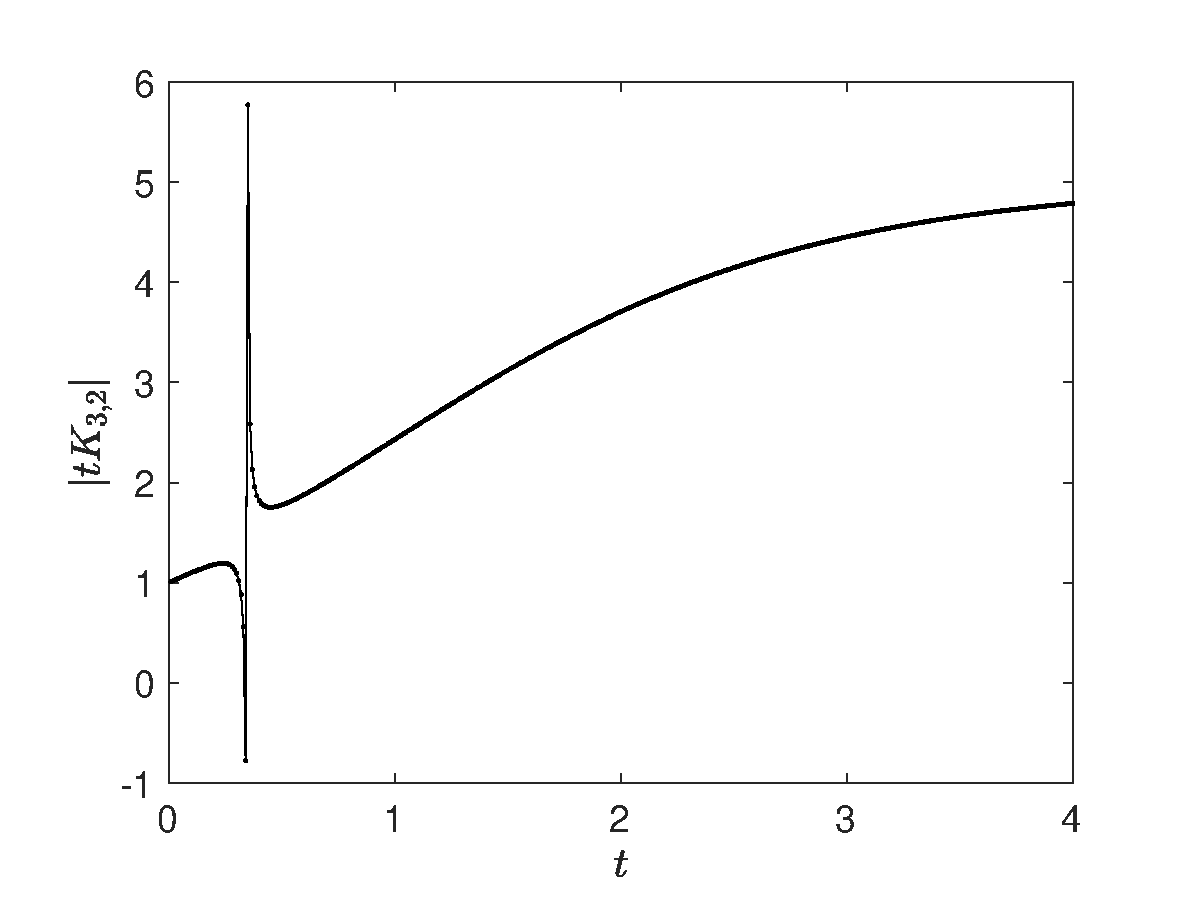
\includegraphics[width=10cm]{K32.eps}\caption{\label{fig:K32magfun}The magnitude function of $K_{3,2}$.}
\end{figure}
\end{frame}

\begin{frame}[allowframebreaks]{Positive definite metric spaces}
For what kinds of spaces does magnitude behave more nicely?

\begin{definition}
A finite metric space $A$ is called \textbf{positive definite} if its similarity matrix $Z_{A}$ is a positive definite matrix.
\end{definition}

\begin{itemize}
\item Positive definite matrices are always invertible, so any positive definite metric space automatically has magnitude.
\item Principal submatrices of positive definite matrices are positive definite so subspaces of positive definite metric spaces also have magnitude.
\item Finite subsets of Euclidean space are positive definite metric spaces.
\end{itemize}

\framebreak

\begin{theorem}[Proposition 2.4.3 of \cite{leinster_magnitude_2011}]\label{thm:variational}
If $A$ is a finite positive definite metric space of $n$ points, then $A$ has magnitude and the magnitude is given by
\begin{equation*}
\vert A \vert = \sup\limits_{v\neq0}\frac{\left(\sum_{a\in A}v_a\right)^2}{v^\ast Z_{A}v}
\end{equation*}
where $v \in \mathbb{R}^n$. The supremum is attained if and only if $v$ is a nonzero scalar multiple of the unique weighting on $A$.
\end{theorem}

\begin{proof}[Idea of proof]\renewcommand{\qedsymbol}{}
Cauchy-Schwarz inequality applied to arbitrary $v$ and weighting $w$.
\end{proof}

\begin{theorem}[Lemma 2.4.10 of \cite{leinster_magnitude_2011}]
If $A$ is a positive definite metric space and $B \subseteq A$, then $\vert B \vert \leq \vert A \vert$.
\end{theorem}

\begin{proof}
Since $A$ is positive definite and $B$ is a subspace, $B$ is also positive definite and both sapces have magnitude. Furthermore, using Theorem \ref{thm:variational} above, we have
\begin{equation*}
\vert B \vert = \sup\limits_{v\neq0}\frac{\left(\sum_{b \in B} v_b\right)^2}{v^\ast Z_{B} v} \leq \sup\limits_{v\neq0}\frac{\left(\sum_{a \in A} v_a\right)^2}{v^\ast Z_{B} v} = \vert A \vert
\end{equation*}
since the space of vectors we are considering for $B$ is a subspace of the space of vectors in consideration for $A$.
\end{proof}

\end{frame}

\begin{frame}[allowframebreaks]{Infinite metric spaces}
\begin{itemize}
\item Want to extend the definition of magnitude to include infinite sets.
\item Idea: approximate by finite subsets.
\item Question: is this way of extending consistent? Is the answer we get independent of the approximation we choose?
\end{itemize}
\end{frame}

\section{Odd-dimensional Euclidean balls}

\begin{frame}[allowframebreaks]{The convex magnitude conjecture}
\end{frame}
\begin{frame}[allowframebreaks]{Asymptotic results}
\end{frame}

\section{Schröder paths}

\begin{frame}[allowframebreaks]{Schröder paths}
\end{frame}

\section{A calculation}

\begin{frame}[allowframebreaks]{Partial results}
\end{frame}

\begin{frame}[plain]
\centerline{Questions?}
\end{frame}

\begin{frame}[plain]
\centerline{Thank you for listening!}
\end{frame}

\begin{frame}[allowframebreaks]{References}
\frametitle{References}
\nocite{*}
\bibliographystyle{amsalpha}
\bibliography{refs.bib}
\end{frame}

%\begin{frame}{Outline}
%  \tableofcontents
%  % You might wish to add the option [pausesections]
%\end{frame}
%
%\section{Introduction to magnitude}
%
%\subsection{Origins in category theory}
%
%\section{Magnitude of a finite metric space}
%
%\subsection{The magnitude function}
%
%\subsection{Positive definite metric spaces}
%
%\section{Infinite metric spaces}
%
%\subsection{Approximation by finite subspaces}
%
%\section{Magnitude of odd-dimensional Euclidean balls}
%
%\subsection{Convex magnitude conjecture}
%
%\subsection{Asymptotic results}
%
%\section{Schroeder paths}
%
%\section{Evaluating the second derivative}
%
%\section{Disjoint $k$-collections with exactly one flat step}
%
%\section{Two flat steps}
%
%\subsection{$\sigma = L$}
%
%\begin{frame}{Some info}
%\begin{equation*}
%\frac{d}{dt}\text{Mag}\left(B_2^d\right) = \frac{1}{2}V_1\left(B_2^d\right)
%\end{equation*}
%\end{frame}
%
%\begin{frame}{Some other info}
%Fill in here
%\end{frame}

\end{document}